% This is based on the LLNCS.DEM the demonstration file of
% the LaTeX macro package from Springer-Verlag
% for Lecture Notes in Computer Science,
% version 2.4 for LaTeX2e as of 16. April 2010
%
% See http://www.springer.com/computer/lncs/lncs+authors?SGWID=0-40209-0-0-0
% for the full guidelines.
%

\documentclass{llncs}
\usepackage{graphicx}
\usepackage[english]{babel}
\usepackage{cleveref}
\begin{document}

\title{PARSIAN 2018\\Extended Team Description Paper}
%
\titlerunning{PARSIAN 2018 ETDP}  % abbreviated title (for running head)
%                                     also used for the TOC unless
%                                     \toctitle is used
%
\author{Mohammad Mahdi Rahimi \and Mohammad Mahdi Shirazi \and \\
Mohammad Amin Najaf Gholyan \and Fateme Hashemi  \and Nadia Moradi \and \\ Fateme Moghadam \and Kian Behzad \and Hamidreza Roudabeh \and Ali Gavahi \and Mohammad Azam Khosravi}
%
\authorrunning{Mohammad Mahdi Rahimi et al.} % abbreviated author list (for running head)
%
%%%% list of authors for the TOC (use if author list has to be modified)
\tocauthor{Mohammad Mahdi Rahimi, Mohammad Mahdi Shirazi,Mohammad Amin Najaf Gholian, Fateme Hashemi , Nadia Moradi, Fateme Moghadam, Kian Behzad, Hamidreza Roudabeh, Ali Gavahi, and Mohammad Azam Khosravi}
%
\institute{	
	Electrical Engineering Department\\
    Amirkabir Univ. Of Technology (Tehran Polytechnic) \\
    424 Hafez Ave. Tehran, Iran\\
	\email{
    	\{mmrahimi,mhmmdshirazi,hashemi96,nadiamoradi,kian.behzad,aligavahi,m.a.khosravi\}@aut.ac.ir 
    },
	\texttt{http://www.parsianrobotics.aut.ac.ir}
}

\maketitle              % typeset the title of the contribution

\begin{abstract}
In this paper, a detailed description of Parsian robots' hardware improvement, as well as new improvements that have been made since last year in the software architecture, is represented. Improvements and developments that seemed innovative and useful in hardware like ball detection sensor, debugger, and self-repair in case of regular fault also improvements in software such as micro-service architecture by ROS, open-loop motion correction and motion profiler, will be discussed in detail.
\keywords{micro-service, ROS, Motion Control, Small Size Robot, ...}
\end{abstract}
%
\section{Introduction}
%
%%% TODO : href and edit is needed %%%
The Parsian small size team, founded in 2005, is organized by Electrical Engineering Department of Amirkabir University of Technology. The purpose of this team is to design and build small size soccer robots compatible with International RoboCup competition rules as a student based project. We have been qualified for twelve consequent years for RoboCup SSL. We participated in years 2008 to 2017 RoboCup competitions. Our most notable achievements were Parsian's first place in RoboCup 2012 SSL's Passing and Shooting, RoboCup 2013 SSL's Navigation challenge and fourth place in RoboCup 2012 and 2017.

This paper has been represented some mechanical changes of Parsian’s robots in Section 2.1 and then features developed for electrical design in Section 2.2 and in Section 3 discussed improvements in control and new microservice architecture.
%

\newpage

\subsection{Team members} %% Just an idea :)
%

%
\section {Hardware}
%
\subsection{Mechanic}
\subsection{Electeronic}
%

\section{Software}
%
\subsection{Control}
 \subsubsection{Open loop motion correction}
This year, in order to achieve perfect motion control, a new learning-based method has been implemented, which fix open-loop motion errors.
In polar coordinates, the robots' movement is expressed as direction angle ($\theta$), velocity (V) and angular velocity ($\omega$). In this method, three offset variables have been added to $\theta$ and $\Omega$, linear velocity was accurate enough and remain without offset. 
At first, a PSO method was implemented with a complicated cost function to optimize multiple variables simultaneously, but after reviewing the results, it was realized that these two parameters ($\theta$ and $\omega$) are almost independent and a simple method can be employed separately, for each parameter. 
One efficient method that can be utilized to optimize a parameter, is Error Back Propagation. It's mainly used in finding weights of neural networks.
The result of this method was satisfying. one instant is provided in the (\ref{fig:1})
\begin{figure}
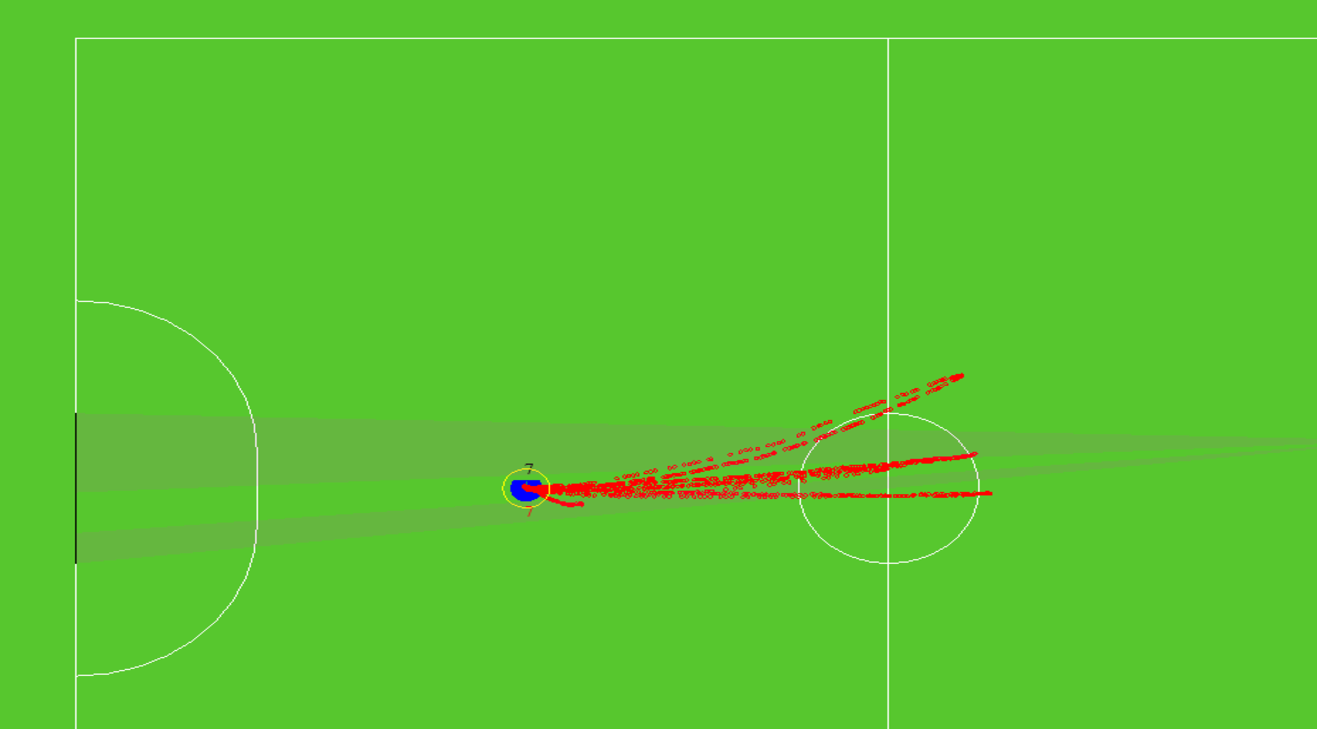
\includegraphics[width=\textwidth]{f1}
\label{fig:1}
\caption{}
\end{figure}
\subsubsection{Angle base deceleration}
The Robot’s maximum deceleration is dependent on the movement angle. previously a constant deceleration had been used for all angles, but this year it was extended to three different decelerations, one for each of the forward, backward and normal angles. Desired deceleration each angle will be calculated by a weighted average, depending on movement angle (\cref{fig:2}).
\begin{figure}
%\centering
%\begin{minipage}{.2\textwidth}
\centering
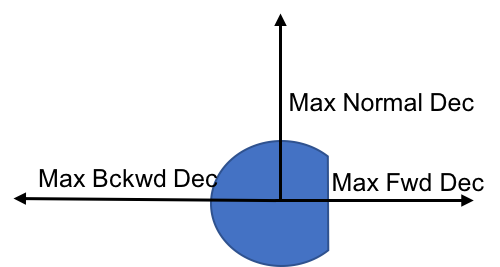
\includegraphics[width=.5\linewidth]{f2}
\label{fig:2}
\caption{}
%\end{minipage}
\centering
%\begin{minipage}{.72\textwidth}
\centering
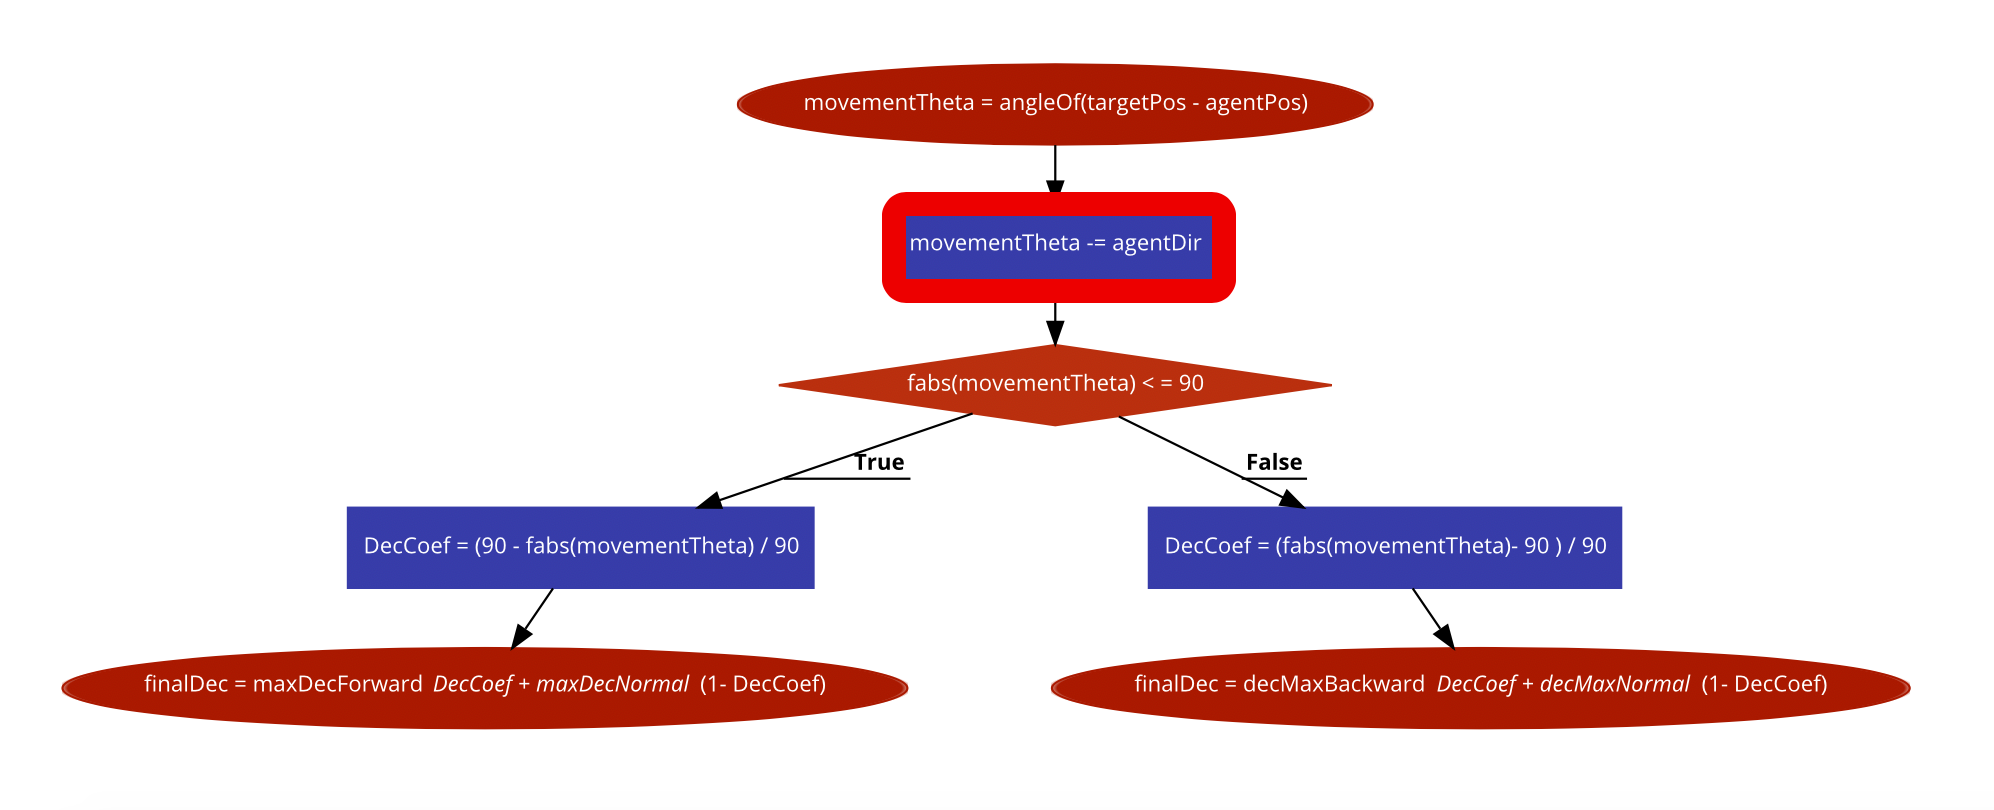
\includegraphics[width=\linewidth]{f3}
\label{fig:3}
\caption{}
%\end{minipage}
\end{figure}
\subsubsection{Motion Profiler}
Motion profiler is a python node that generates robot task for a robot to move in different distances, angles, and directions. Then it records vision data, robot’s motion data and dispatched commands. There are other scripts that collect useful information from these raw data that are represented below.
\begin{enumerate}  
\item Robot velocity-time table of each motion
\item Remaining distance-time table of each motion
\item  Command velocity-time table of each motion
\end{enumerate}
Then it calculates some useful information including:
\begin{enumerate}  
\item Total delay by calculating time shift between speed and command 
\item Time needed for a robot to move from each point to another with four-dimensional regression on the raw data
\end{enumerate}

\subsubsection{Obstacle Avoidance} 
Parsian has been using ERRT algorithm for years, which is a random algorithm that is often used in real-time approaches. This year, in order to decrease the number of collisions and also minimize the travel time, a new approach for obstacle avoidance has been developed. this method does not intend to change RRT implementation or propose a new way to avoid obstacles. it’s rather about how to define the obstacles space.
This method is based on opponent robots’ capabilities:
\begin{enumerate}  
\item Maximum Deceleration
\item Maximum Velocity
\item Agility Factor
\item Current velocity 
\end{enumerate}
A probability area can be chosen for a certain upcoming time interval.
    If the probability area for opponent robots and future position of our robot  overlap, then the obstacle avoidance try to avoid that common space.
Agility Factor represents by how many degrees, the movement direction of a robot can change, during a specified time in its maximum velocity.

\subsection{System Architecture}
\subsubsection{Latency}
\begin{table}
\caption{Result of Parsian}
\begin{center}
\begin{tabular}{r@{\quad}rcl}
\hline
\multicolumn{1}{c}{\rule{0pt}{12pt}Year} & \multicolumn{2}{c}{Result}\\[2pt]
\hline\rule{0pt}{12pt}
RoboCup 2014  &     Round Robin& \\
RoboCup 2015  &     Lucky Loser& \\
RoboCup 2016  &     Lucky Loser& \\
RoboCup 2017  &     4th Place  & \\
RoboCup 2018  & 	1st Place  & \\[2pt]
\hline
\end{tabular}
\end{center}
\end{table}
%

\section{Conclusion}
         AI and behavior will be change according to this year rules, and major work on passing and receiving in dynamic play that started from 2016 will be used in a real game since calculating time with new Kalman and motion profiler is enough accurate to execute passing.
     
    Last year, auto-profiler and log analyzer were proven to be very useful. In Iran Open \& Robocup 2017 auto-profiling and analyzing greatly reduced the amount of team setup time which allowed us to focus more on strategic planning. Although the main software that was built in 2008 and improved each year, has given us successful competition result for the last years, result summarized in table2, but changing old monolithic software architecture to distributed in this year was another enormous work that makes a great advantage to develop, test and debug system. Also the huge number of open-source project help to not reinventing the wheel. This year, Parsian hardware's changes aim to stabilize robots with detecting and monitoring their faults and in control part, motion controller improved greatly by improving Kalman, open-loop calibration and profiler.


\begin{table}
\caption{Result of Parsian}
\begin{center}
\begin{tabular}{r@{\quad}rl}
\hline
\multicolumn{1}{c}{\rule{0pt}{12pt}Year} & \multicolumn{2}{c}{Result}\\[2pt]
\hline\rule{0pt}{12pt}
RoboCup 2014  &     Round Robin& \\
RoboCup 2015  &     Lucky Loser& \\
RoboCup 2016  &     Lucky Loser& \\
RoboCup 2017  &     4th Place  & \\
RoboCup 2018  & 	1st Place  & \\[2pt]
\hline
\end{tabular}
\end{center}
\end{table}
%
%

%
% ---- Bibliography ----
%
\begin{thebibliography}{5}
%
\bibitem {clar:eke}
Clarke, F., Ekeland, I.:
Nonlinear oscillations and
boundary-value problems for Hamiltonian systems.
Arch. Rat. Mech. Anal. 78, 315--333 (1982)

\bibitem {clar:eke:2}
Clarke, F., Ekeland, I.:
Solutions p\'{e}riodiques, du
p\'{e}riode donn\'{e}e, des \'{e}quations hamiltoniennes.
Note CRAS Paris 287, 1013--1015 (1978)

\bibitem {mich:tar}
Michalek, R., Tarantello, G.:
Subharmonic solutions with prescribed minimal
period for nonautonomous Hamiltonian systems.
J. Diff. Eq. 72, 28--55 (1988)

\bibitem {tar}
Tarantello, G.:
Subharmonic solutions for Hamiltonian
systems via a $\bbbz_{p}$ pseudoindex theory.
Annali di Matematica Pura (to appear)

\bibitem {rab}
Rabinowitz, P.:
On subharmonic solutions of a Hamiltonian system.
Comm. Pure Appl. Math. 33, 609--633 (1980)

\end{thebibliography}




\end{document}
